\documentclass{article}
\usepackage{graphicx}
\usepackage{amsmath}
\usepackage{array}
\usepackage[font=small, labelfont={sf,bf}, margin=1cm]{caption}
\usepackage{tabularx}
\usepackage{amssymb}
\usepackage{esint}


\date{Due: Nov 6 Edit: \today}
\title{NPRE 321 HW 5}
\author{James Liu}

\begin{document}
\maketitle
\begin{itemize}
    \item [1.] \
    \begin{itemize}
        \item [a)] \
        \begin{figure*}[h]
            \centering
            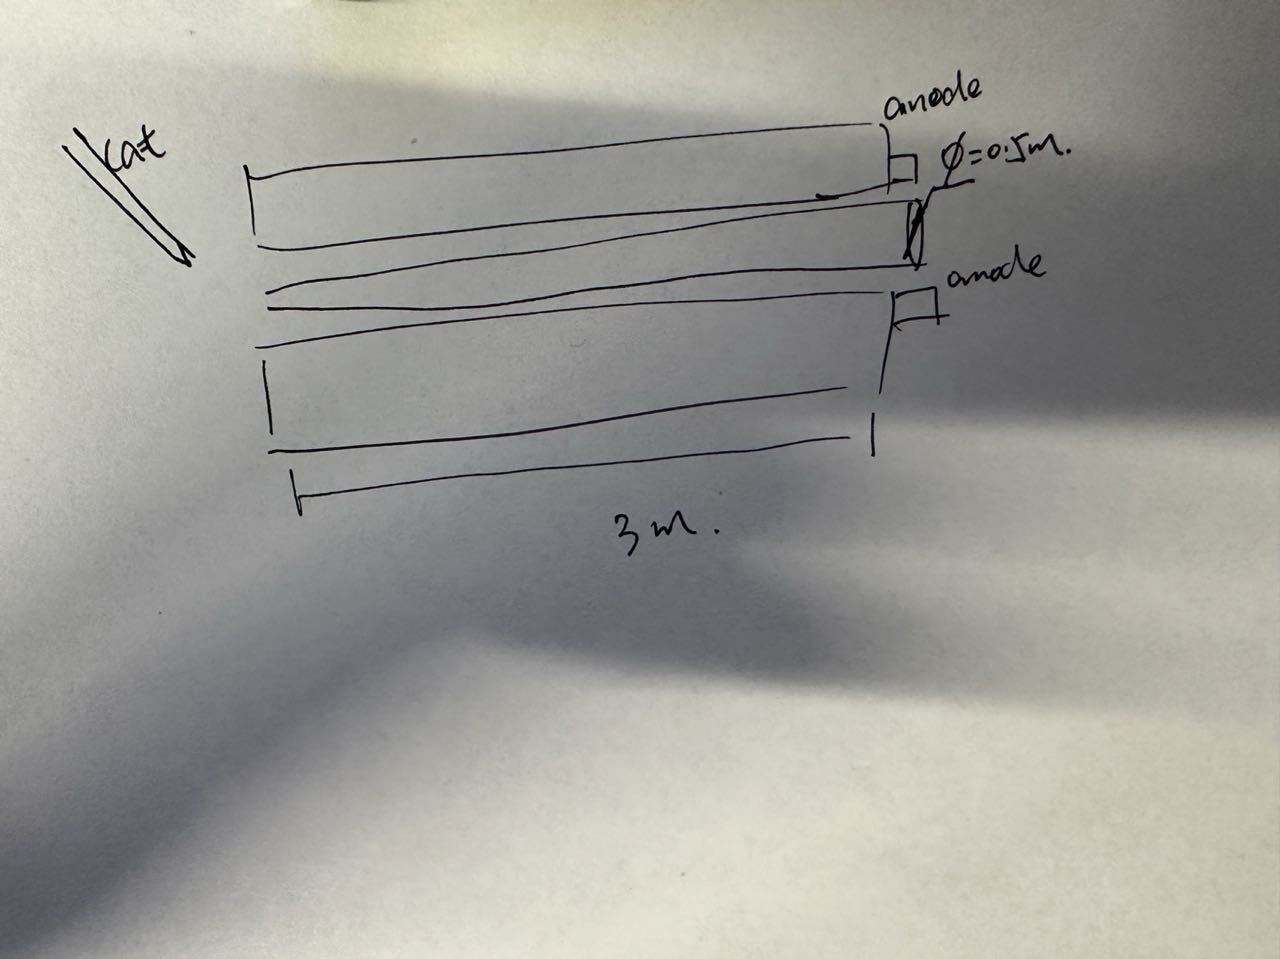
\includegraphics[scale=0.25]{figure/fig1_npre321_hw5_.jpeg}
        \end{figure*}
        \item [b)] \
        \begin{align*}
            \tau =\frac{R^2}{2D_b}&=\frac{R^2}{2\left(\frac{kT_e}{16eB}\right)}\\
            &=\frac{0.25}{\frac{1.602\times 10^{-19}\times 5}{8\times 1.602\times 10^{-19}\times1}}\\
            &=0.4 \text{s}
        \end{align*}
        \item [c)] \
        \begin{align*}
            v^2 &=2E/m\\
            v&=\sqrt{2\frac{kT}{m}}\\
            &=\sqrt{2\times \frac{1.602\times 10^{-19}\times 5}{1.007276\times 1.661\times 10^{-27}}}\\
            &= 3.094\times 10^4 \text{ m/s}\\
            v_{\bot }&=\frac{1}{\sqrt2}v = 2.1878\times 10^{4} \text{m/s}\\
            r &=\frac{vm}{qB} \\
            &=\frac{2.1878\times 10^{4}\times1.007276\times 1.661\times 10^{-27}}{1.602\times 10^{-19}\times 1}\\
            &=3.66043\times 10^{-23} \text{m}
        \end{align*}
        \item [d)]\
        \begin{align*}
            \lambda_D &= \sqrt{\frac{\varepsilon_0 kT}{ne^2}}\\
            &=\sqrt{\frac{8.854\times 10^{-12}\times 1.602\times 10^{-19}\times 5}{10^{20}\times (1.602\times 10^{-19})^2}}\\
            &=1.6623\times 10^{-6} \text{m}\\
            \Lambda  &=12\pi n \lambda_D^3\\
            &=12\pi 10^{19}\times(1.6623\times 10^{-6})^3\\
            &=1731.82\\
            \lambda_0 &=3.4\times 10^{13}\frac{T^2}{n\ln(\Lambda)}\\
            &=3.4\times 10^{13}\times \frac{5^2}{10^{19}\ln(1731.82)}\\
            &=1.13\times 10^{-5}
        \end{align*}
        \item [e)]\
        The mean free path will dominant collisions. \\ \(3/1.13\times 10^{-5} = 2.63\times 10^5\)
    \end{itemize}
    \item [2.]\
    \begin{itemize}
        \item [Semiconductor:]Plasmas are extensively used in micro-fabrication processes, which involve patterning materials to create integrated circuits. Key processes include:
        Plasma Etching: Removing unwanted material to create patterns on silicon wafers. For instance, \(CF_4\) gas is used to etch silicon (Si), where the plasma breaks molecular bonds, releasing free fluorine (F) atoms. These atoms react with silicon to form volatile 
        \(SiF_4\) gas, which can be pumped away. To ensure thorough etching, \(O_2\) is added to remove carbon residues, although careful control of gas mixtures is needed to avoid unwanted reactions.
        Plasma Deposition: Used to lay down thin films. This can be achieved through methods like:
        \\
        Sputtering: A plasma ionizes gas (like argon), and the energetic ions bombard a target material, ejecting atoms that coat a substrate.\\
        Chemical Vapor Deposition (CVD): Plasma assists in breaking down gases to deposit materials at lower temperatures, enhancing efficiency and creating chemically reactive species.
        \item [Surface Treatment:]
        Plasma-Assisted Sputtering: Using reactive sputtering, materials like titanium (Ti) are combined with gases such as nitrogen (\(N_2\)) to create compounds like titanium nitride (TiN). This compound, often golden in color, coats tools for increased wear resistance.
        \\
        Ion Implantation: Energetic ions from the plasma embed into the surface, altering its properties. High-energy plasma ions can also sputter away surface contaminants or create textured surfaces for specific applications.
        \item [source type:]
        \begin{itemize}
            \item [1.]Direct Current (DC) Plasmas: Simple to set up, with low density and temperature, ideal for straightforward applications. However, they tend to have high contamination and are used where uniformity is not critical.
            \item [2.]Radiofrequency (RF) Plasmas: Commonly used in plasma processing, including:
            Capacitively Coupled Plasma (CCP): Simple to construct, suitable for processes without magnetic fields, but with lower plasma density.
            \\
            Inductively Coupled Plasma (ICP): Higher density and more uniform, making it suitable for etching and deposition where precision is needed. However, these setups are complex and require extensive cooling and pumping.
            \\
            Helicon Plasmas: Specialized ICPs with higher densities and uniform profiles, used in applications requiring fine control over plasma properties.
            \item [3.] Magnetron Plasmas: Use microwave energy to create a high-density plasma near a cathode, ideal for sputtering. They allow for the deposition of metals, oxides, and insulating materials with uniform layers, although plasma density is relatively low.
            \item [4.] Vacuum Arc Discharges: Produce fully ionized plasma for high-rate deposition with low substrate temperatures. However, they risk contamination and require magnetic filtering.
        \end{itemize}
    \end{itemize}
\end{itemize}
\end{document}